\documentclass{homeworg}

\title{Housing Price in Scotland}
\author{Alif Sussardi}
\usepackage{hyperref}
\usepackage[section]{placeins}
\hypersetup{
    colorlinks=true,
    linkcolor=blue,
    filecolor=blue,      
    urlcolor=blue,
}
\begin{document}
\graphicspath{ {./figure/} }
\maketitle

\section{Introduction}
\subsection{Background}
Scotland is one of the least densely populated area in the UK. It making a big chunk of the UK land, which comprises of about 32\% of the total land area in the UK. However, it only contributes to 8.2\% total population.[1] The most populated cities: Glasgow and Edinburgh are astonishing, with large population of immigrants and tourists. In 2016 alone, there are 2.6 million foreign visitor and 11.5 million domestic, which contributes to £6 billion GDP, 4.5\% Scottish GDP. This tourism industry is contributing to about 207,000 employment, which makes about 8\% of Scottish workforce[2]. \par
This boom in tourism causing housing market very competitive for residents which has to compete with tourist. During festival season, July-August, the competition even more significant, when the landlords/homeowner try to rent their property to festival goer. As a resident of Edinburgh, where the rent is increasing every year and finding place to stay becoming more difficult, it is makes sense for me to understand how housing price is determined. \par
Other than touristy Edinburgh and Glasgow where Hotels, restaurants and coffee place is blossoming, there are other places such as Aberdeen and Dundee which are relying on other source of income. 

\subsection{Aim}
The Aim for this report is to determine whether the Housing Price is determined exclusively by location, population density or also contributed by venues nearby. Also, by looking at the most common venue nearby, we could estimate what investment that can be done in a particular region.

\subsection{Interest}
From this report, property buyer will be informed, whether the purchase is with good value for a certain areas. Also, investors will also get insight on which place is best for investing in a particular business and areas such as opening coffee shop, pub, restaurant or more of manufacturing plant or just simply sporting venue.

\section{Data Acquisition and Cleaning}
\subsection{Data Sources}
This report used house price of October 2020 and October 2019 as comparison. The Scotland house price of October 2020 was an excel file, obtained from the website of \href{https://www.ros.gov.uk/__data/assets/excel_doc/0010/173575/RoS_monthly-house-price-statistics_tables_Oct-2020.xlsx}{Register of Scotland} [3]. The excel file contains comprehensive data of house sales in Scotland, along with several supporting information including Average Price, Total Value and Sale Volume. Each local authority, or later will be used interchangeably with county, is identified with Local Authority Code, which contains 1 digit of letter, followed by 8 digits of number. The letter represents the nation, in the case of Scotland, it is "S", and 8 digits of number are unique. \par
The comparing data of house price if October 2019 is available from the same source, ROS [4]. It can be found in \href{https://www.ros.gov.uk/__data/assets/excel_doc/0007/171385/RoS_quarterly-house-price-statistics_tables_2020-21-Q2_July-to-September-2020.xlsx}{new file} as well as in the previous file. This file contains large dataset, including average price, sales volume, house type, \textit{etcetera}. \par
The geospatial coordinate (latitude and longitude) of each local authority is assigned using geolocator package. This geospatial coordinate will be used to find venues available in eah local authority. \par
The Scotland geospatial JSON was collected from a GitHub by \href{https://github.com/martinjc/UK-GeoJSON/raw/master/json/administrative/sco/lad.json}{martinjc}[5]. This JSON file was used to draw choropleth map of scotland according to the data that has been obtained from the last paragraphs. \par
To obtain the population density, the land area data was also obtained from \href{https://www.ros.gov.uk/__data/assets/excel_doc/0016/162016/property-market-report-2019-2020.xlsx}{ROS}[6], and the population data was obtained from \href{https://www.ons.gov.uk/file?uri=\%2fpeoplepopulationandcommunity\%2fpopulationandmigration\%2fpopulationestimates\%2fdatasets\%2fpopulationestimatesforukenglandandwalesscotlandandnorthernireland\%2fmid2019april2020localauthoritydistrictcodes/ukmidyearestimates20192020ladcodes.xls}{Office of National Statistics (ONS)}[7].
\subsection{Data Cleaning}
The data were downloaded and identified find the correct sheets to load, as well as their correct header, rows and columns. Pandas library was used for this particular task. The data was also selected based on the Scotland code identifier, to get the local authority of interest. The data from multiple sources are selected and combined using merge and/or join syntax based on local authority code. This local authority code is essential as unique identifier, as using the local authority name often cause erroneous merging due to multiple versions of writing the name. \par
The Scotland geospatial JSON data was downloaded and used to plot choropleth map. The data JSON data however, contains some errors in the local authority assignment to the correct county. Therefore, a correction has to be performed to assign correct local authority code. This can be done using conventional notepad, or using a more sophisticated text editor such as notepad++. The failure to correct this JSON file will result in the erroneous area not coloured properly, or shaded completely black for the lack of data in the dataframe.\par
The latitude and longitude data, however, were assigned to specific local authority name, not using the code. The reason behind this is that the geolocators package, search for name of a county to get coordinates. However, the use of local authority code has not been attempted. \par
The name and number of venue were searched from the county coordinate using Forsquare API within 2.5 km radius. The radius of 2.5 km was chosen with an assumption that it is a reasonable distance to go around city either by walking, cycling, car or public transport. This method, however, lack in the precision of the town/township location, since the latitude and longitude were searched using the county name, which is not necessarily represent the name of the most populous area in the county. Later on, a county without available venues will be dropped, as it is a sign that the coordinate were assigned to rural areas, and will not be used for comparison.
\subsection{Feature Selection}
The feature of the main dataframe contains 32 rows of county/local authorities, with relevant columns:
\begin{itemize}
    \item \textbf{index} - contains Local Authority Code,
    \item \textbf{LocalAuthority} - contains County name,
    \item \textbf{AveragePrice} - average housing price of October 2020 in GBP,
    \item \textbf{SalesVolume} - number of housing sales in October 2020,
    \item \textbf{TotalValue} - total money transacted for Housing sales in October 2020 in GBP,
    \item \textbf{latitude},
    \item \textbf{longitude},
    \item \textbf{AveragePrice19} - average housing price of October 2019 in GBP,
    \item \textbf{UrbanAreas} - in ${Hectare}^2$,
    \item \textbf{RuralAreas} - in ${Hectare}^2$,
    \item \textbf{TotalArea} - in ${Hectare}^2$, and
    \item \textbf{Population}.
\end{itemize}
Population density (\textbf{PopDensity}) column was added by computing the Population/TotalArea. The Urban Density (\textbf{UrbanDensity}) was added by computing the Population/UrbanAreas, under assumption that the population in each county reside in the rather urban part of the county. 
\section{Exploratory Data Analysis}
\subsection{Mapping of Population density and Average Housing Price}
The population density of each county is assigned into the choropleth map of Scotland, as shown in \textbf{Figure \ref{fig:fig1}}. From the figure, we can clearly see that the population density is high at the City of Edinburgh, Aberdeen City, Dundee City, Glasgow City and its supporting areas. This is expected as those cities are where the population mostly resides, which contributes to big chunk of population. \par
\begin{figure}[!h]
    \centering
    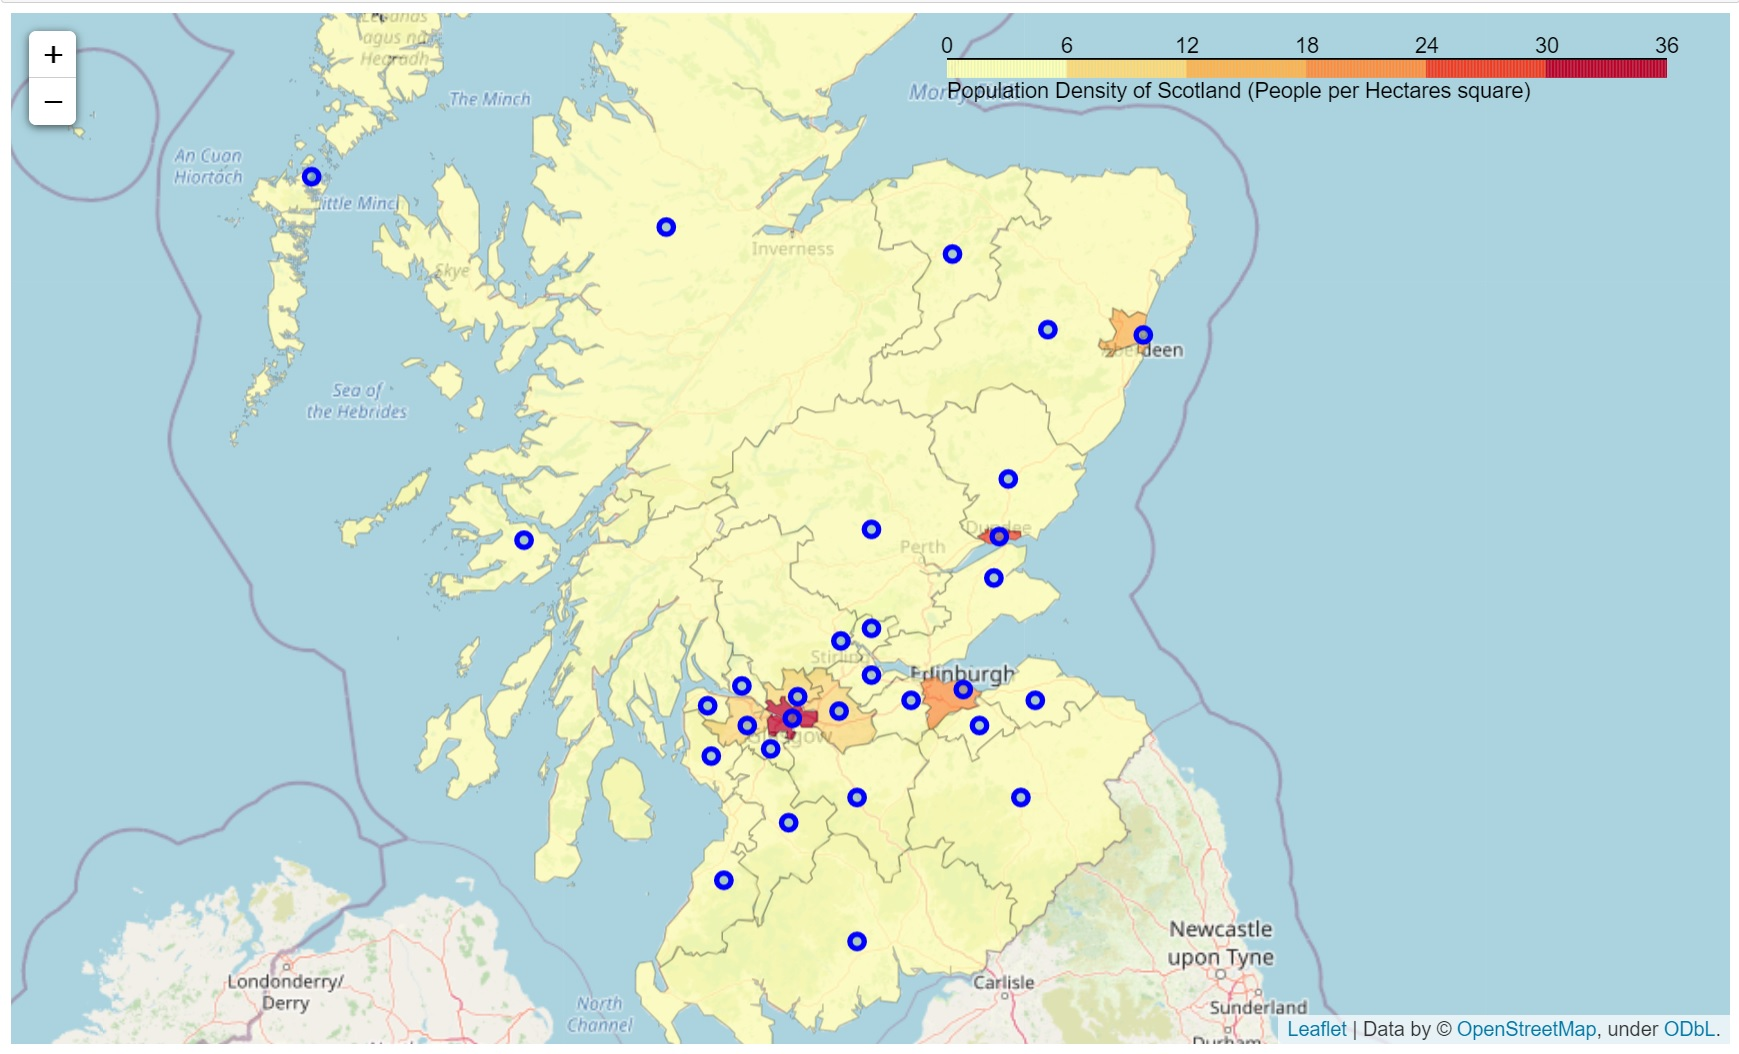
\includegraphics[scale=0.7]{figure/Figure_1_Populat_on_Density_Map.jpg}
    \caption{The Population Density Map of Scotland}
    \label{fig:fig1}
\end{figure}
\FloatBarrier
The question would be whether the population density will affect its Housing Price. It can be seen from \textbf{Figure \ref{fig:fig2}} that the price is high in the City of Edinburgh and East Renfrewshire, which is supporting area for Glasgow City. Glasgow city itself is not considered as a city with expensive housing price according to the figure. The pricing in the other region, however, does not seems to follow any pattern. \par
Average price in Aberdeen and Dundee seems to be lower than its surrounding areas, which raise a question what really is affecting the price?
\begin{figure}[!h]
    \centering
    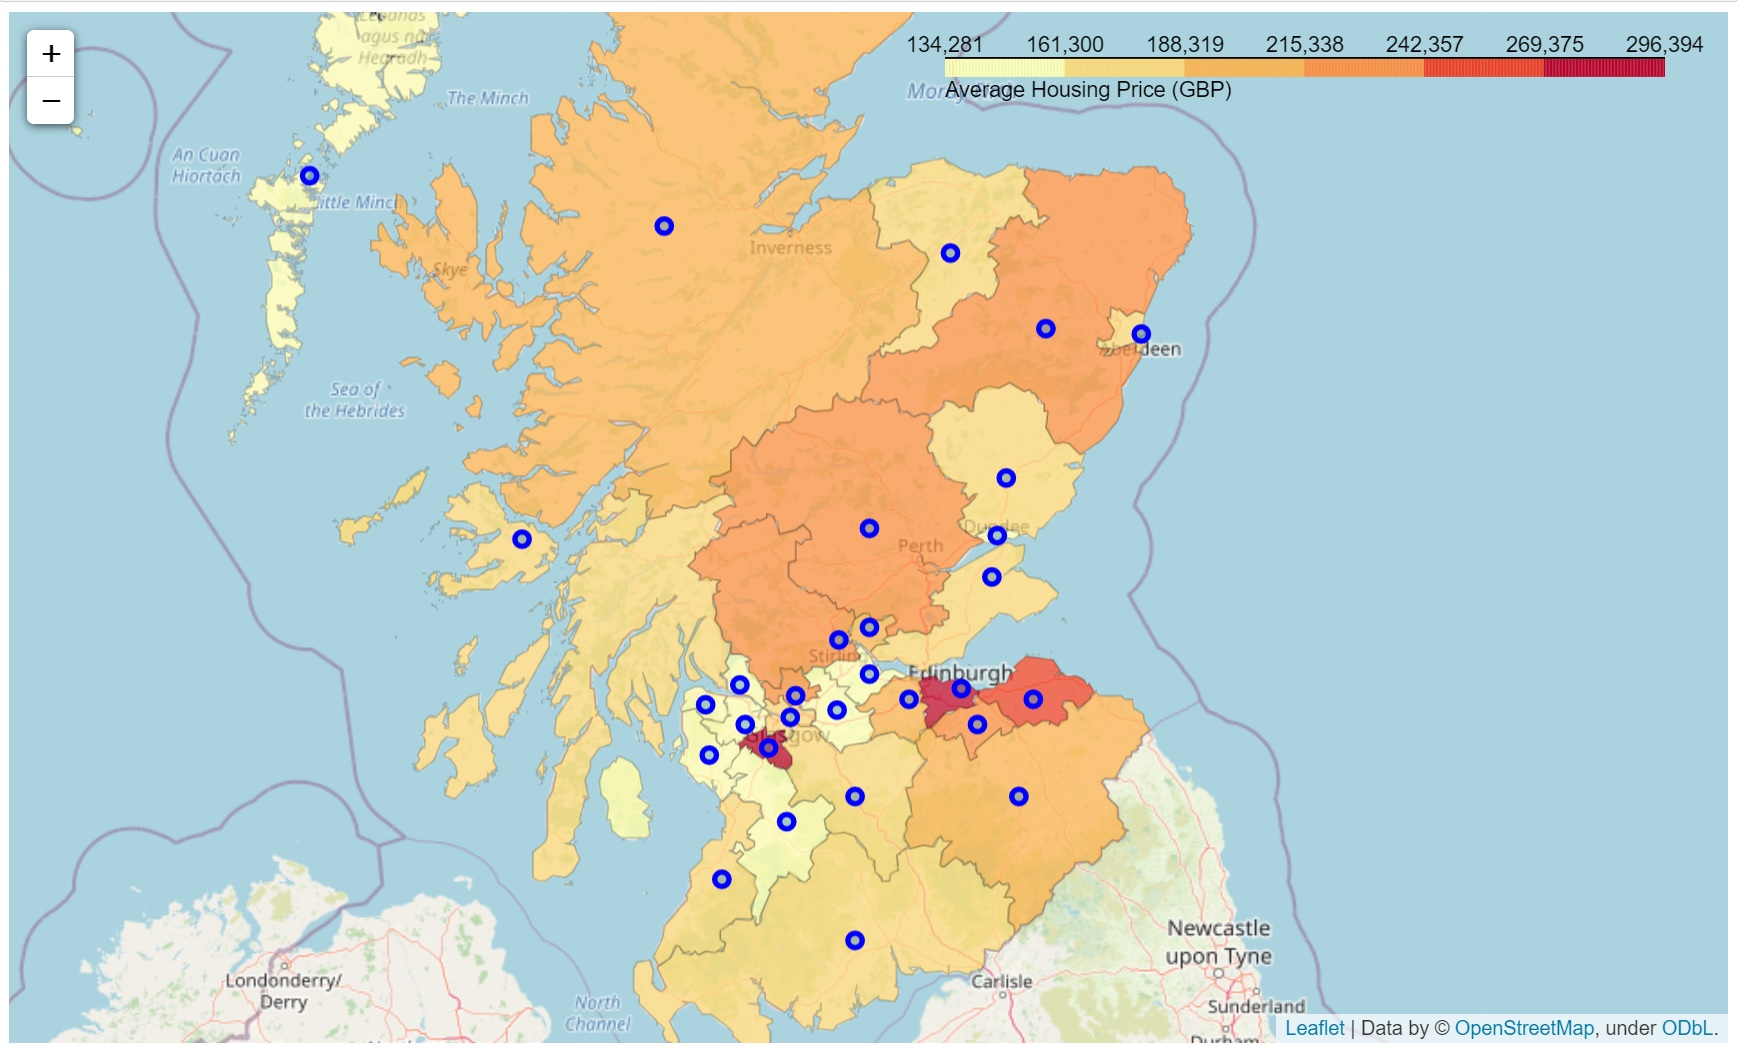
\includegraphics[scale=0.7]{figure/Figure_2_Average_Housing_Price_Map.jpg}
    \caption{The average housing Price of Scotland}
    \label{fig:fig2}
\end{figure}
\FloatBarrier
\subsection{Looking at the Obvious}
One assumption is that the higher the population, the more the value of transaction and the number of sales. To see whether this is true, we can plot it in a scatter plot and see the relationship.
\subsubsection{Population vs. Total Transaction Value}
The Total Transaction Value can be seen clearly depending on the number of population, as shown in \textbf{Figure \ref{fig:fig3}}, with increase of Total value of 100 million, in every increase of 432 people. This will also make each person contribute to about 231,000 GPB spent for a house in Scotland. One city that is standout with the most Total Value Transacted is unsurprisingly the City of Edinburgh, with the total Value Transacted of about 350 million GBP, way higher than the projected Total Value Transacted for its population at about 200 million GBP.
\begin{figure}[!h]
    \centering
    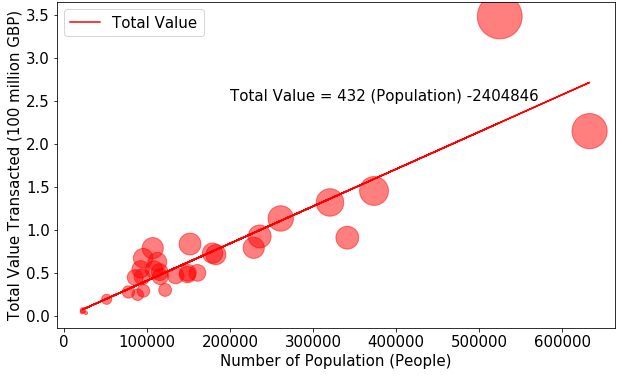
\includegraphics[scale=0.6]{figure/Figure_3_The_Obvious_PopulationVSTotalValue.png}
    \caption{\textbf{The Obvious}: Population vs. Total Transaction
    Value}
    \label{fig:fig3}
\end{figure}
\FloatBarrier
\subsubsection{Population vs. Number of Sales}
It only makes sense that with the increase number of population, the number of transaction/sales will also increase. This can be seen clearly in \textbf{Figure \ref{fig:fig4}}, where each 1000 people in the region, contribute to 2 sales. This also means that in a group of 1000 people, 2 people is buying house, in October 2020. The city of Edinburgh, that in \textbf{Figure \ref{fig:fig3}} shown to have 350 million GBP transaction, contribute to about 1200 sales, which makes the average price is about 290,000 per house. The property in the City of Edinburgh is significantly more expensive than other county of about 220,000 GBP per property.
\begin{figure}[!h]
    \centering
    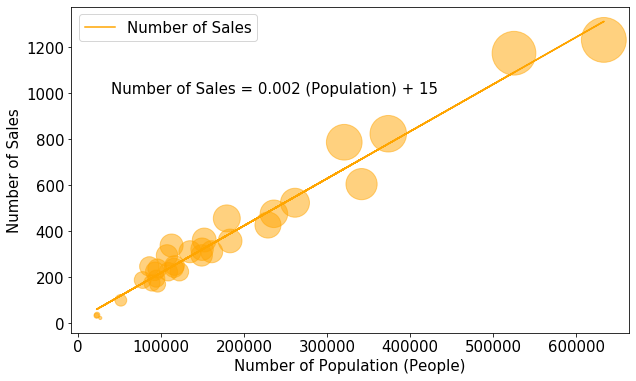
\includegraphics[scale=0.6]{figure/Figure_4_The_Obvious_PopulationVSNumberofSales.png}
    \caption{\textbf{The Obvious}: Number of Sales as a function of Population}
    \label{fig:fig4}
\end{figure}
\FloatBarrier
\subsection{Things That Are Not So Obvious}
Question will rise whether other factor will affect the Property price in Scotland, such as Population Density or Number of Venues.
\subsubsection{Population Density vs. Average Price}
To see whether the more dense the population, the more expensive the average price of a house. To answer this question, data can be plotted accordingly, as shown in  \textbf{Figure \ref{fig:fig5}}. The Average Price of 2020 and 2019 are included, and show there is an overall increase in house price from 2019 to 2020.\par However, the relationship between the population density and average price is rather conclusive. Although the slope of the plot showing positive slope, the spread of the data are large, causing the relationship between the two is unclear.\par
\begin{figure}[!h]
    \centering
    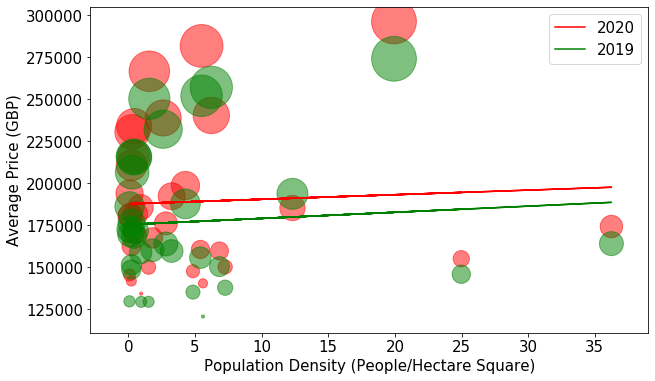
\includegraphics[scale=0.6]{figure/Figure_5_Not_so_Obvious_PopulationDensityVSAveragePrice.png}
    \caption{Average Price as a function of Population Density}
    \label{fig:fig5}
\end{figure}
\FloatBarrier
But what about Average Price as a function of Urban Density? It should be noted that: It is assumed that majority of the population live in the urban area, therefore the population density should be depending on the urban areas, but not total area which include significant area for conservation, \textit{etcetera}. This is shown in \textbf{Figure \ref{fig:fig6}}, where we can see that the more densely populated urban area, the higher the price. It can be shown as well from the trend-line that in 2019, the difference between low and high density population is steeper than in 2020.\par
\begin{figure}[!h]
    \centering
    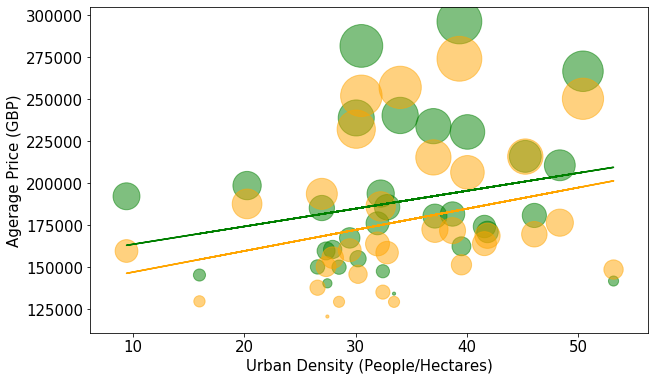
\includegraphics[scale=0.6]{figure/Figure_6_Not_so_Obvious_UrbanDensityVSAveragePrice.png}
    \caption{Average Price as a function of Urban Density}
    \label{fig:fig6}
\end{figure}
\FloatBarrier
\subsubsection{Number of Venues vs. Average Price}
In order to see whether number of venues and the type of of venues affecting the price, I need to look for the venues first. This task can be done using Forsquare API. The Forsquare, however, has a limitation in that maximum number of venues that can be obtained for each coordinates, which is only 100. Therefore, when a county has more than 100 venues, it will maxed out at 100. The venues were browsed within 2.5 km radius. The number of venues for each county can be seen in \textbf{Figure \ref{fig:fig7}}.
\begin{figure}[!h]
    \centering
    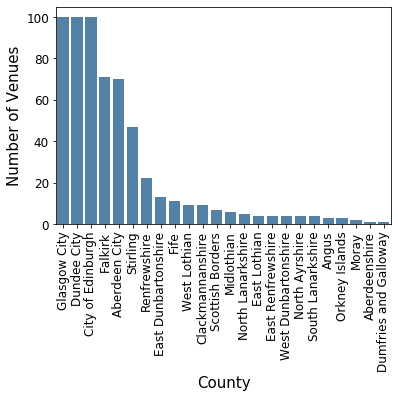
\includegraphics[scale=0.9]{figure/Figure_7_County_vs_NumOfVenues.png}
    \caption{Number of Venues in each County}
    \label{fig:fig7}
\end{figure}
\FloatBarrier
The Average housing price then can be plotted as a function of number of venues, as can be seen in \textbf{Figure \ref{fig:fig8}}. As we can see as well that the number of venues within 2.5 km radius does not seems to affect the average price of housing in Scotland. There seems to be no correlations between the two parameters. But it is interesting to see that the most neighborhood has less than 20 venues. The 3 county with most venues are the City of Edinburgh, Glasgow City and Dundee City. 
\begin{figure}[!h]
    \centering
    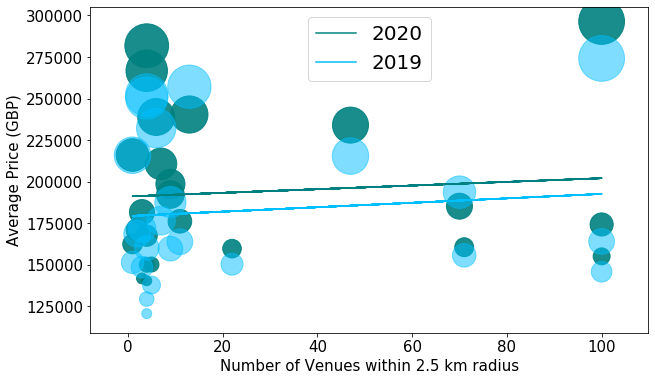
\includegraphics[scale=0.6]{figure/Figure_10b_NumOfVenues_VS_AveragePrice_yearly.png}
    \caption{Average Price as a function of Number of Venues}
    \label{fig:fig8}
\end{figure}
\FloatBarrier
The city of Edinburgh is indeed has the highest housing price. However, the second and third cities that has the most venues: Dundee and Glasgow, are not even in the top 10 list of county with most expensive housing price, as shown in \textbf{Figure \ref{fig:fig9}}. 
\begin{figure}[!h]
    \centering
    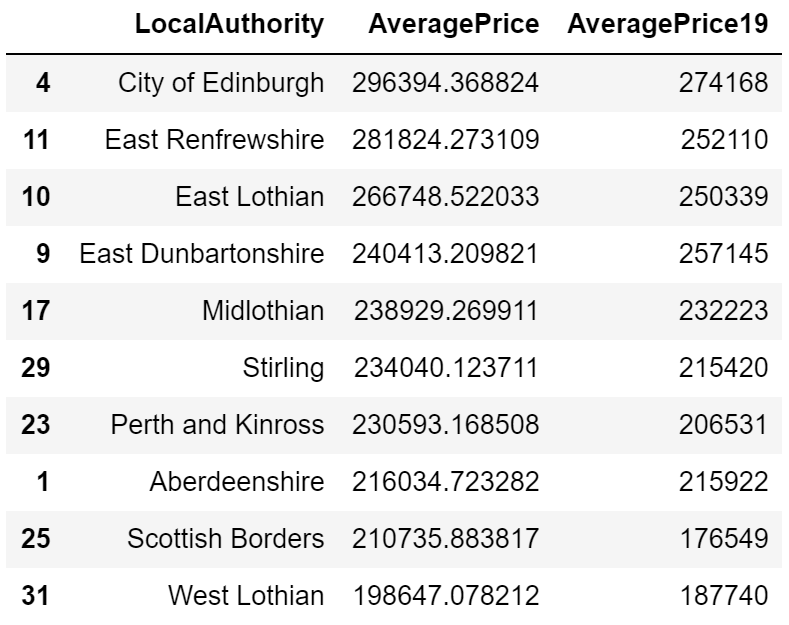
\includegraphics[scale=1]{figure/Table_of_10_highest_average_price.png}
    \caption{Table of County with highest Housing Average Price}
    \label{fig:fig9}
\end{figure}
\FloatBarrier
The venues then identified and grouped and assigned to each county. The 1st, 2nd and 3rd most common venues are identified, and shown in \textbf{Figure \ref{fig:fig10}}. It can be seen that the most common venue is Hotel, and followed by drinking places such as Coffee shop, Pub and Bar. This could indicate that indeed counties in Scotland are having characteristics of touristy place.
\begin{figure}[!h]
    \centering
    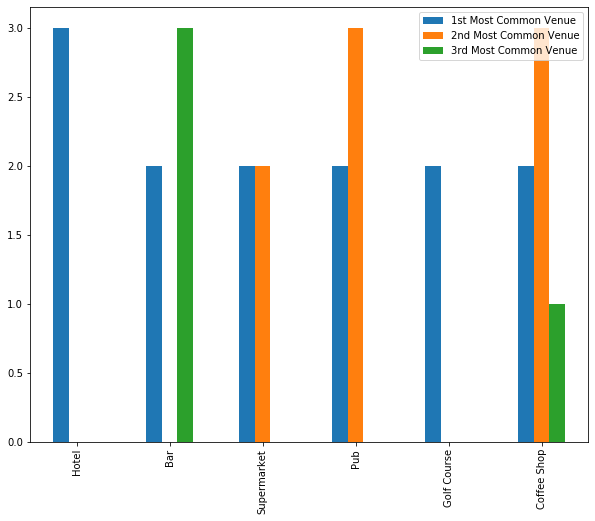
\includegraphics[scale=0.6]{figure/Figure_8_Venues_Most_Common_Barplot.png}
    \caption{The 1st, 2nd and 3rd most common venues}
    \label{fig:fig10}
\end{figure}
\FloatBarrier
During the time of COVID-19, tourism industry is hit hard. The question would be whether the housing price is affected? from previous figures, it seems that overall housing price in Scotland does not really affected. But what about region with many venues that support tourism? Do they affected? To answer this question, a column of \textbf{PriceIncrease} is calculated by subtracting \textbf{AveragePrice} with \textbf{AveragePrice19}, and then plot it as a function of Number of Venues, as shown in \textbf{Figure \ref{fig:fig11}}. 
\begin{figure}[!h]
    \centering
    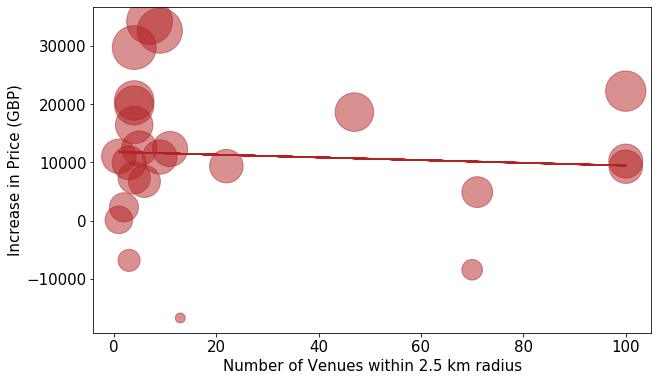
\includegraphics[scale=0.6]{figure/Figure_11_NumOfVenues_VS_IncreaseInPRice.png}
    \caption{Housing Price Increase from October 2019 to October 2020 as a function of Number of Venues}
    \label{fig:fig11}
\end{figure}
\FloatBarrier
From \textbf{Figure \ref{fig:fig11}}, it can be seen that the more the county has venues, the less the increase of housing price from October 2019 to October 2020. The reason for this could be due to the impact of COVID-19 to the tourism industry. The more an area has venues, the harder it got hit. This could also suggest that the area where the economy is not depending on venues, the more resilient the housing price. 
\section{Clustering}
To find characteristics of county based on its venues, a clustering can be made based on the venues nearby. This characteristic of county will be important as it gives information about what to invest in a county and where should we buy property considering circumstance such as upcoming pandemic, \textit{etcetera}.
In this case, the clustering was using k-means clustering, as it contains quite large parameters; there are 158 features (venues category), and k-means guarantee convergence. It can also provides irregular shape of clustering such as elliptical shape, relative to its centroid. This is very beneficial, remembering that there are 158 parameters to cluster.
\subsection{Looking for the Best k}
To find the best k, or number of cluster, it is best to find a change in gradient of the SSE vs number of k , as shown in \textbf{Figure \ref{fig:fig12}}. It could be seen from the figure that there is a change in gradient around k = 3. Therefore k = 3 is used to cluster the county based on venues features.
\begin{figure}[!ht]
    \centering
    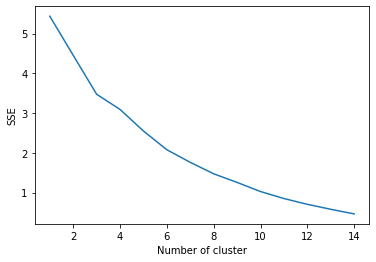
\includegraphics[scale=0.7]{figure/Figure_9_No_Cluster_VS_SSE.png}
    \caption{Square Sum Error (SSE) as a function of number of k}
    \label{fig:fig12}
\end{figure}
\FloatBarrier
\subsection{Clustering Based on Venue}
The clustering were carried out using k = 3, and the cluster number were assigned to each county. These counties with assigned cluster number then plotted in a choropleth map containing \% Urban Area, to see whether there is a pattern. \par
\textbf{Figure \ref{fig:fig13}} shows that there is a clear pattern, with the points of cluster no. 0 appearing at the place with dense urban areas. The cluster no.1 Show a close proximity with cluster no. 0, and cluster no 2, appears to be in a more rural areas.\par
\begin{figure}[!ht]
    \centering
    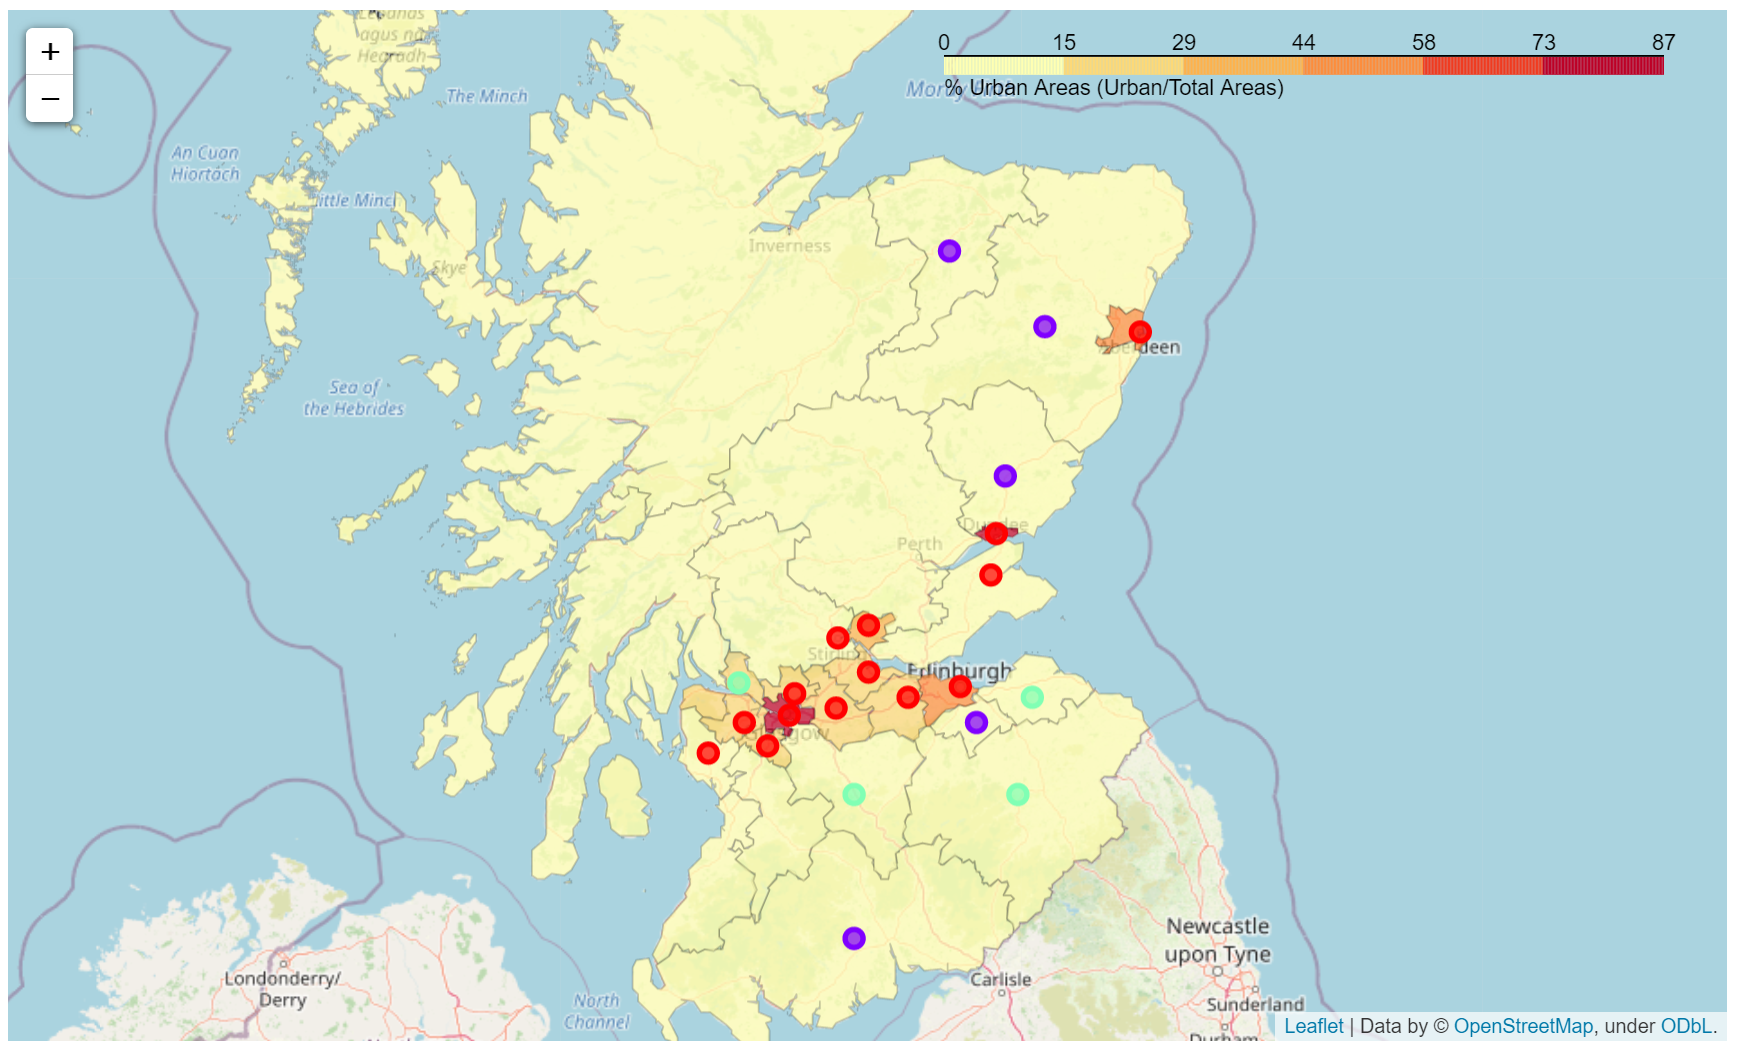
\includegraphics[scale=0.7]{figure/Figure_9_Clustered_with_percent_urban_areas.png}
    \caption{Map of Scotland showing population density in color with assigned cluster number in points. Red, green and purple circles represent the cluster no. 0, 1 and 2, respectively.}
    \label{fig:fig13}
\end{figure}
To see what similarity between county within the cluster, tables can be shown as follow.\par
\begin{figure}[!ht]
    \centering
    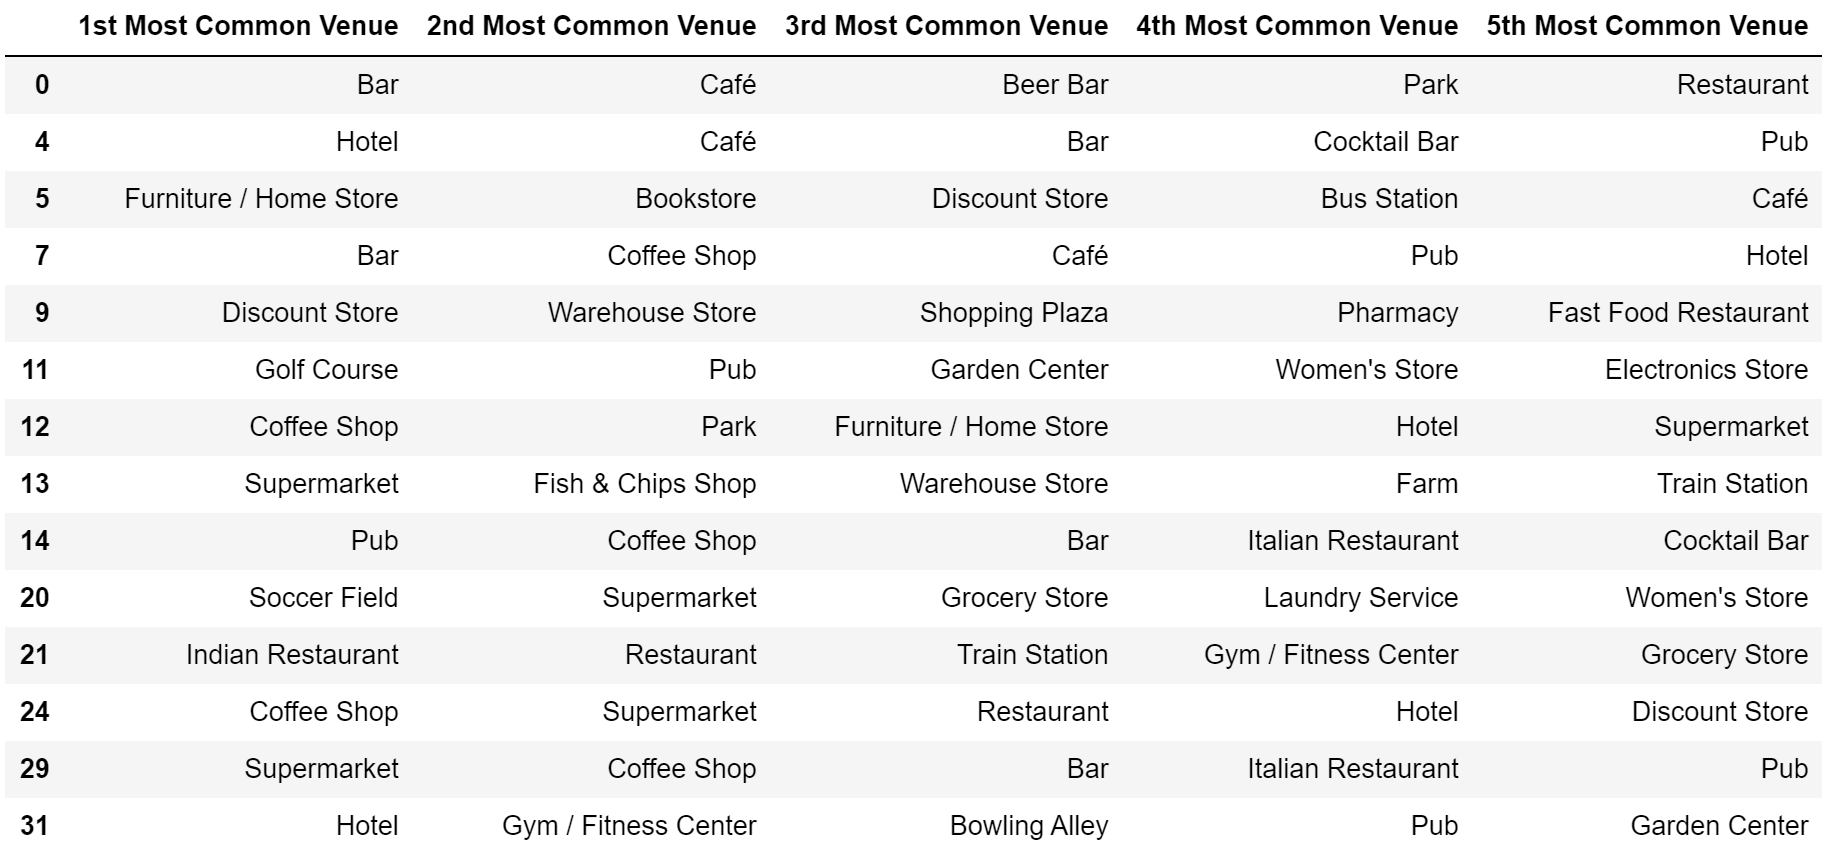
\includegraphics[scale=0.8]{figure/Table_of_Cluster_0.png}
    \caption{Cluster No.0}
    \label{fig:clust0}
\end{figure}
\FloatBarrier \par
From the \textbf{Figure \ref{fig:clust0}}, it can be seen that Cluster No. 0  shows drinking places such as Bar, Pub, Coffee shop as well as Pubs, This is characteristics of touristy place. This cluster, as has been described previously, the housing price is rather susceptible to the COVID-19, therefore, it is best not to invest to this area when there is a sign of upcoming pandemic. To invest in drinking place might also be not too wise, if the product is not outstanding, since there will be quite competition from a massive population of drinking places. However, if investor really confident about their drinking/beverage products, it can be tested in this area, since it has many of customer, especially tourist, during normal day.\par 
\begin{figure}[!ht]
    \centering
    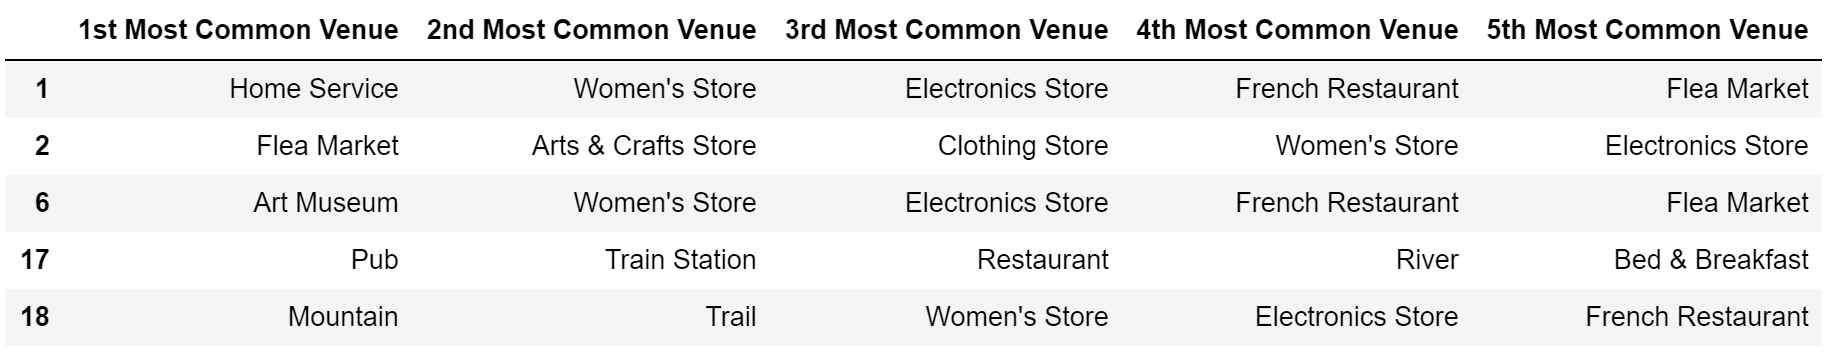
\includegraphics[scale=0.8]{figure/Table_of_Cluster_1.png}
    \caption{Cluster No.1}
    \label{fig:clust1}
\end{figure}
\FloatBarrier \par
From the \textbf{Figure \ref{fig:clust1}}, it shown that Cluster No.1 shows area with more Stores and Flea Market and less of drinking places. This indicates that this area specialised in supporting the touristy places. They sell subsistence such as food or food ingredients an not so fancy products (i.e. flea market). Workers from the touristy are may also live in this area. Therefore, this place might not be to susceptible to COVID-19 pandemic, or any upcoming economic disturbances, since this area only directly deal with tourist. A cheap takeout place would be interesting to open in this area, with touristy worker as target customer. Opening a grocery store might not be wise since it will directly compete with big player in this area.\par
\begin{figure}[!ht]
    \centering
    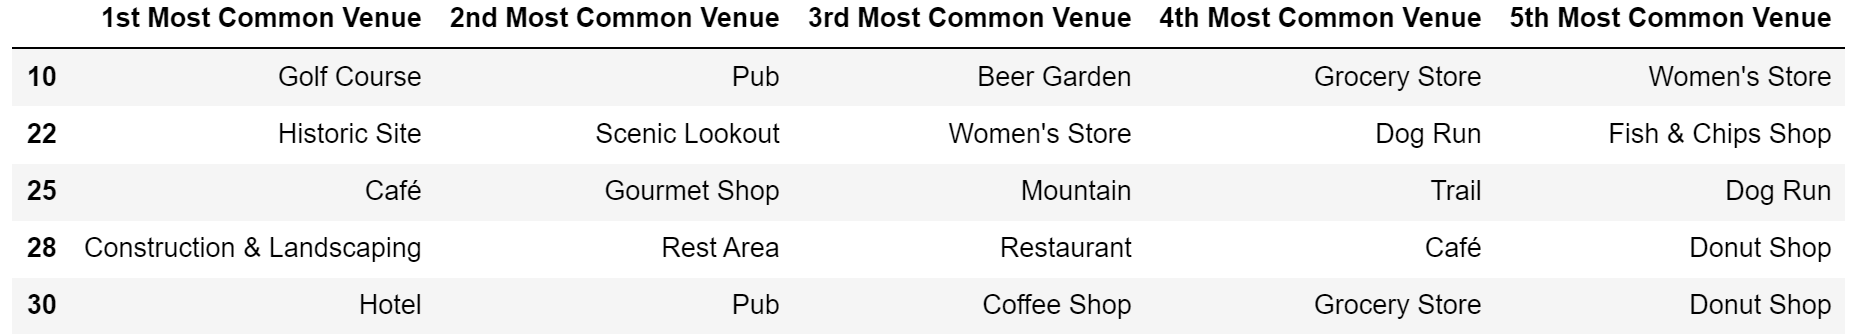
\includegraphics[scale=0.8]{figure/Table_of_Cluster_2.png}
    \caption{Cluster No. 2}
    \label{fig:clust2}
\end{figure}
The final cluster, No. 2, show a characteristics of rather rural area with few takeouts, and more represented by outdoor venues and its supporting venues. This area has the most resilience housing price against COVID-19 pandemic as its main purpose is for residential area, probably to workers that not related to tourism business. To open grocery store or home depot might be lucrative in this area. To invest in housing for a long term investment might also be worth doing, since any economic disturbance give little effect on it price. \par
The question is still, what about the price comparison of these cluster? As we can see from \textbf{Figure \ref{fig:clustPrice}}, the cluster 0 (touristy place) has the highest average price, since there is a constant demand for tourist accommodation and supporting activity. Followed by the cluster 1 (supporting area for tourism), and the last is the residential area of cluster 2. Each cluster or area has its own perks in investing on different area of investments as has been explained in previous paragraphs.\par
\begin{figure}[!ht]
    \centering
    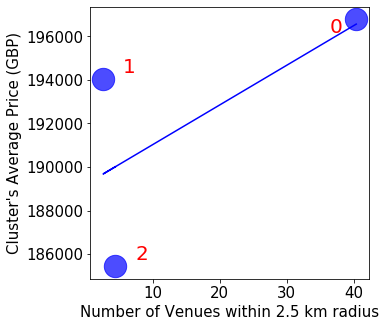
\includegraphics[scale=0.7]{figure/Clusters_Average_Price.png}
    \caption{Average Housing Price of each cluster as a function of number of venues}
    \label{fig:clustPrice}
\end{figure}
\section{Conclusions}
To Conclude, this report successfully get an idea why Housing Price in certain area in Scotland is expensive. It is, in fact not depending on the number of cluster, but rather the type, with touristy area with its amenities give rise to Housing price. It also worth noting that the price in this touristy area is fragile to an economic disturbance related to tourism such as COVID-19 pandemic. While the rural residential area, steadily increase its price each year.\par
In touristy area, it might not too wise to invest in drinking place, since there is a tough competition with other business in beverage. Unless, the beverages product is really outstanding and the characteristics is liked by the inhabitants and demography of tourists. In supporting of touristy area, however, it might be good to invest in a cheap takeout place, with touristy worker as target customer, there is also less venue in this area and it might be wise to invest in property, regardless of economic disturbances in tourism, (the touristy business workers might still need to be nearby, and they still pay rent!). In rural residential area, however, it might be good to invest in property, if investor are concern about economic disturbances, as this area provides investment security in property. To invest in grocery store and food ingredients might be good, but it might need extra effort for promotion, since its quite sparsely populated area. \par
\section{Future Work}
It will be interesting to map the demography of the tourists to see the tourist preference, whether in type of food, beverages, accommodation and attractions. This will determine what type of investment will be lucrative in the certain area, off course once the COVID-19 pandemic has passed. 
\section{References}
1. https://en.wikipedia.org/wiki/Demography\_of\_Scotland \par
2. https://www2.gov.scot/Topics/Statistics/Browse/Tourism\#:~:text=The\%20number \%20of \%20domestic\%20tourism,2006\%20total\%20(15.6\%20million). \par
3. https://www.ros.gov.uk/\_\_data/assets/excel\_doc/0010/173575/RoS\_monthly- house-price-statistics\_tables\_Oct-2020.xlsx \par
4. https://www.ros.gov.uk/\_\_data/assets/excel\_doc/0007/171385/RoS\_quarterly- house-price-statistics\_tables\_2020-21-Q2\_July-to-September-2020.xlsx \par
5. https://github.com/martinjc/UK-GeoJSON/raw/master/json/administrative/ sco/lad.json \par
6. https://www.ros.gov.uk/\_\_data/assets/excel\_doc/0016/162016/property-market- report-2019-2020.xlsx \par
7. https://www.ons.gov.uk/file?uri=\%2fpeoplepopulationandcommunity\%2fpopulationand migration\%2fpopulationestimates\%2fdatasets\%2fpopulationestimatesforukenglandandwal esscotlandandnorthernireland\%2fmid2019april2020localauthoritydistrictcodes/ukmidyear estimates20192020ladcodes.xls \par
\end{document}
